\documentclass[12pt]{article}
\usepackage{setspace, graphicx, fullpage, amssymb, amsmath, epsfig, natbib, array, multirow, hyperref}
\usepackage{amsfonts, bm} 
\usepackage{dcolumn}
\usepackage{subfigure, float} 
\usepackage[margin=0.75in]{geometry} 
\usepackage{verbatim}
\usepackage{url}
\usepackage{enumerate}
\newcolumntype{d}[1]{D{.}{.}{#1}} 

\begin{document}
	
	
\begin{center}
		\Large Update 24 January 2017, cont.
\end{center}

I wrote this document after the other since I couldn't get more tables to properly place themselves on the page. Sorry for any inconsistencies between the two

In this document, tables 1 through 3 on pages 1 through 4 contain the regression tables for the Senate with $p$-value thresholds of 0.01 and 0.05 as well as the House replication table. These are followed by the extremism figures 1 through three found on pages 5 through 7 which are ordered in the same way as the tables. Finally, I tried separately modeling Southern and Non-Southern Democrats to see if this was what was driving the results. The results are mixed for other Democrats depending on our $p-$value threshold, but more ideologically extreme Southern Democrats are less likely to respond to party calls in our model.

The results of the previous weeks in the Senate are robust to a higher $ p $-value threshold for party calls. This should be unsurprising given the previous week's findings. Further, corrections to the variables and multiple checks to ensure they were being coded correctly have maintained the result that more ideologically extreme Democrats are \textit{less} responsive to the party calls we identify. 

\begin{table}[ht]
	\begin{center}
		\begin{tabular}{l c c c c }
			\hline
			& Democrats & Republicans & Majority & Minority \\
			\hline
			ideological\_extremism & $-3.931^{***}$ & $2.820^{***}$ & $-1.427^{*}$   & $1.605^{*}$    \\
			& $(0.687)$      & $(0.564)$     & $(0.659)$      & $(0.625)$      \\
			chair                  & $-1.652^{*}$   & $-2.172^{**}$ & $-1.817^{**}$  &                \\
			& $(0.644)$      & $(0.733)$     & $(0.661)$      &                \\
			pfrate100              & $0.824^{***}$  & $0.895^{***}$ & $0.889^{***}$  & $0.870^{***}$  \\
			& $(0.034)$      & $(0.031)$     & $(0.034)$      & $(0.034)$      \\
			pres\_vote\_share      & $30.828^{***}$ & $-5.643$      & $15.589^{***}$ & $16.808^{***}$ \\
			& $(2.848)$      & $(3.180)$     & $(2.558)$      & $(3.063)$      \\
			south                  & $-3.324^{***}$ & $0.216$       & $0.676$        & $-1.563^{*}$   \\
			& $(0.635)$      & $(0.594)$     & $(0.550)$      & $(0.618)$      \\
			power\_committee       & $-0.455$       & $1.432$       & $0.420$        & $0.139$        \\
			& $(0.907)$      & $(0.952)$     & $(0.919)$      & $(1.051)$      \\
			vote\_share            & $-6.152^{*}$   & $4.650$       & $1.168$        & $-3.431$       \\
			& $(2.548)$      & $(2.894)$     & $(2.650)$      & $(2.885)$      \\
			female                 & $-0.575$       & $1.337$       & $-0.354$       & $2.444^{*}$    \\
			& $(0.860)$      & $(1.146)$     & $(0.962)$      & $(1.088)$      \\
			afam                   & $4.228$        & $-7.687$      & $1.393$        & $-1.934$       \\
			& $(3.270)$      & $(4.399)$     & $(5.302)$      & $(3.162)$      \\
			latino                 & $-1.069$       & $-5.641^{*}$  & $-1.634$       & $-2.254$       \\
			& $(2.740)$      & $(2.850)$     & $(2.506)$      & $(3.448)$      \\
			up\_for\_reelection    & $-0.812$       & $0.008$       & $0.144$        & $-1.351^{*}$   \\
			& $(0.493)$      & $(0.553)$     & $(0.516)$      & $(0.591)$      \\
			seniority              & $0.012$        & $0.152$       & $0.107$        & $0.113$        \\
			& $(0.071)$      & $(0.086)$     & $(0.085)$      & $(0.079)$      \\
			freshman               & $-0.525$       & $0.379$       & $0.649$        & $0.618$        \\
			& $(0.679)$      & $(0.796)$     & $(0.722)$      & $(0.804)$      \\
			retiree                & $2.115^{*}$    & $0.947$       & $2.273^{*}$    & $1.416$        \\
			& $(1.071)$      & $(1.032)$     & $(1.098)$      & $(1.097)$      \\
			best\_committee        & $0.212$        & $-0.181$      & $0.050$        & $0.096$        \\
			& $(0.151)$      & $(0.168)$     & $(0.156)$      & $(0.181)$      \\
			leader                 & $-0.881$       & $-0.038$      & $0.067$        & $-0.553$       \\
			& $(0.844)$      & $(0.802)$     & $(0.852)$      & $(0.887)$      \\
			(Intercept)            & $4.595$        & $8.268^{*}$   & $-0.688$       & $1.795$        \\
			& $(3.244)$      & $(3.578)$     & $(3.442)$      & $(3.721)$      \\
			\hline
			R$^2$                  & 0.629          & 0.658         & 0.589          & 0.649          \\
			Adj. R$^2$             & 0.623          & 0.652         & 0.582          & 0.643          \\
			Num. obs.              & 1037           & 951           & 1048           & 842            \\
			RMSE                   & 7.160          & 7.435         & 7.428          & 7.598          \\
			\hline
			\multicolumn{5}{l}{\scriptsize{$^{***}p<0.001$, $^{**}p<0.01$, $^*p<0.05$}}
		\end{tabular}
		\caption{Senate $ p < 0.01 $}
	\end{center}
\end{table}



\begin{table}[ht]
	\begin{center}
		\begin{tabular}{l c c c c }
			\hline
			& Democrats & Republicans & Majority & Minority \\
			\hline
			ideological\_extremism & $-1.029$       & $1.362^{**}$  & $0.524$        & $1.767^{**}$   \\
			& $(0.578)$      & $(0.485)$     & $(0.506)$      & $(0.549)$      \\
			chair                  & $0.060$        & $-1.603^{*}$  & $-1.723^{**}$  &                \\
			& $(0.557)$      & $(0.649)$     & $(0.526)$      &                \\
			pfrate100              & $0.832^{***}$  & $0.865^{***}$ & $0.890^{***}$  & $0.793^{***}$  \\
			& $(0.029)$      & $(0.027)$     & $(0.026)$      & $(0.030)$      \\
			pres\_vote\_share      & $18.068^{***}$ & $9.586^{***}$ & $14.195^{***}$ & $11.811^{***}$ \\
			& $(2.474)$      & $(2.816)$     & $(2.021)$      & $(2.782)$      \\
			south                  & $-2.322^{***}$ & $0.109$       & $0.979^{*}$    & $-2.088^{***}$ \\
			& $(0.552)$      & $(0.527)$     & $(0.438)$      & $(0.560)$      \\
			power\_committee       & $-1.384$       & $0.529$       & $-0.485$       & $-0.240$       \\
			& $(0.787)$      & $(0.844)$     & $(0.732)$      & $(0.953)$      \\
			vote\_share            & $-4.249$       & $-0.415$      & $-1.491$       & $-2.918$       \\
			& $(2.211)$      & $(2.570)$     & $(2.107)$      & $(2.617)$      \\
			female                 & $-1.758^{*}$   & $-1.209$      & $-2.330^{**}$  & $0.970$        \\
			& $(0.746)$      & $(1.014)$     & $(0.766)$      & $(0.987)$      \\
			afam                   & $3.880$        & $-6.240$      & $0.782$        & $-1.420$       \\
			& $(2.834)$      & $(3.899)$     & $(4.220)$      & $(2.867)$      \\
			latino                 & $-2.892$       & $-8.058^{**}$ & $-2.842$       & $-7.983^{*}$   \\
			& $(2.376)$      & $(2.528)$     & $(1.995)$      & $(3.129)$      \\
			up\_for\_reelection    & $-0.722$       & $-0.405$      & $-0.098$       & $-1.154^{*}$   \\
			& $(0.427)$      & $(0.490)$     & $(0.411)$      & $(0.536)$      \\
			seniority              & $-0.136^{*}$   & $-0.068$      & $0.063$        & $-0.122$       \\
			& $(0.061)$      & $(0.076)$     & $(0.068)$      & $(0.072)$      \\
			freshman               & $-1.268^{*}$   & $-0.428$      & $-0.325$       & $-0.969$       \\
			& $(0.587)$      & $(0.706)$     & $(0.574)$      & $(0.730)$      \\
			retiree                & $1.836^{*}$    & $0.649$       & $1.493$        & $1.413$        \\
			& $(0.928)$      & $(0.915)$     & $(0.874)$      & $(0.995)$      \\
			best\_committee        & $0.260^{*}$    & $-0.072$      & $0.113$        & $0.027$        \\
			& $(0.131)$      & $(0.149)$     & $(0.124)$      & $(0.164)$      \\
			leader                 & $-0.349$       & $1.522^{*}$   & $0.630$        & $-0.035$       \\
			& $(0.732)$      & $(0.710)$     & $(0.678)$      & $(0.804)$      \\
			(Intercept)            & $7.023^{*}$    & $5.855$       & $0.297$        & $11.788^{***}$ \\
			& $(2.810)$      & $(3.186)$     & $(2.740)$      & $(3.357)$      \\
			\hline
			R$^2$                  & 0.693          & 0.689         & 0.716          & 0.659          \\
			Adj. R$^2$             & 0.688          & 0.684         & 0.711          & 0.653          \\
			Num. obs.              & 1037           & 951           & 1048           & 842            \\
			RMSE                   & 6.206          & 6.594         & 5.913          & 6.892          \\
			\hline
			\multicolumn{5}{l}{\scriptsize{$^{***}p<0.001$, $^{**}p<0.01$, $^*p<0.05$}}
		\end{tabular}
		\caption{Senate $ p < 0.05 $}
	\end{center}
\end{table}

\begin{table}
	\begin{center}
		\begin{tabular}{l c c c c }
			\hline
			& Democrats & Republicans & Majority & Minority \\
			\hline
			(Intercept)            & $-6.86^{***}$ & $-0.45$       & $4.84^{***}$  & $4.42^{**}$   \\
			& $(1.40)$      & $(1.70)$      & $(1.46)$      & $(1.49)$      \\
			ideological\_extremism & $4.52^{***}$  & $6.25^{***}$  & $7.38^{***}$  & $7.23^{***}$  \\
			& $(0.24)$      & $(0.25)$      & $(0.24)$      & $(0.24)$      \\
			pfrate100              & $0.95^{***}$  & $0.71^{***}$  & $0.77^{***}$  & $0.65^{***}$  \\
			& $(0.02)$      & $(0.01)$      & $(0.02)$      & $(0.01)$      \\
			pres\_votepct          & $0.04^{***}$  & $0.23^{***}$  & $0.13^{***}$  & $0.25^{***}$  \\
			& $(0.01)$      & $(0.01)$      & $(0.01)$      & $(0.01)$      \\
			south                  & $-2.62^{***}$ & $1.59^{***}$  & $0.92^{***}$  & $-1.73^{***}$ \\
			& $(0.21)$      & $(0.25)$      & $(0.20)$      & $(0.24)$      \\
			votepct                & $0.03^{***}$  & $0.02$        & $-0.02^{**}$  & $-0.02$       \\
			& $(0.01)$      & $(0.01)$      & $(0.01)$      & $(0.01)$      \\
			female                 & $0.63^{*}$    & $-1.34^{**}$  & $-1.31^{***}$ & $0.97^{**}$   \\
			& $(0.29)$      & $(0.43)$      & $(0.32)$      & $(0.35)$      \\
			afam                   & $-0.62$       & $0.55$        & $-3.59^{***}$ & $-3.53^{***}$ \\
			& $(0.35)$      & $(2.24)$      & $(0.43)$      & $(0.50)$      \\
			latino                 & $-1.37^{**}$  & $-0.03$       & $-0.94$       & $-2.66^{***}$ \\
			& $(0.43)$      & $(0.87)$      & $(0.50)$      & $(0.57)$      \\
			seniority              & $-0.10^{***}$ & $-0.17^{***}$ & $-0.08^{**}$  & $-0.11^{**}$  \\
			& $(0.03)$      & $(0.04)$      & $(0.03)$      & $(0.03)$      \\
			freshman               & $0.24$        & $1.46^{***}$  & $0.26$        & $0.48$        \\
			& $(0.29)$      & $(0.35)$      & $(0.28)$      & $(0.36)$      \\
			bestgrosswart          & $-0.02$       & $0.17^{***}$  & $0.01$        & $0.10^{***}$  \\
			& $(0.02)$      & $(0.02)$      & $(0.02)$      & $(0.02)$      \\
			leader                 & $0.47$        & $1.62^{**}$   & $1.50^{**}$   & $1.22^{*}$    \\
			& $(0.50)$      & $(0.58)$      & $(0.52)$      & $(0.53)$      \\
			power                  & $1.44^{***}$  & $-0.30$       & $0.72^{**}$   & $0.03$        \\
			& $(0.23)$      & $(0.28)$      & $(0.22)$      & $(0.29)$      \\
			chair                  & $2.52^{***}$  & $3.37^{***}$  & $1.13^{**}$   & $3.65$        \\
			& $(0.41)$      & $(0.61)$      & $(0.35)$      & $(3.72)$      \\
			\hline
			R$^2$                  & 0.75          & 0.59          & 0.74          & 0.62          \\
			Adj. R$^2$             & 0.75          & 0.59          & 0.74          & 0.62          \\
			Num. obs.              & 4676          & 3759          & 4839          & 3596          \\
			RMSE                   & 6.03          & 6.69          & 5.98          & 6.43          \\
			\hline
			\multicolumn{5}{l}{\scriptsize{$^{***}p<0.001$, $^{**}p<0.01$, $^*p<0.05$}}
		\end{tabular}
		\caption{House Replication Table}
	\end{center}
\end{table}

\begin{figure}[ht]
	\caption{Figure 2, Ideological Extremism, Senate $ p < 0.01 $}
	\centering
	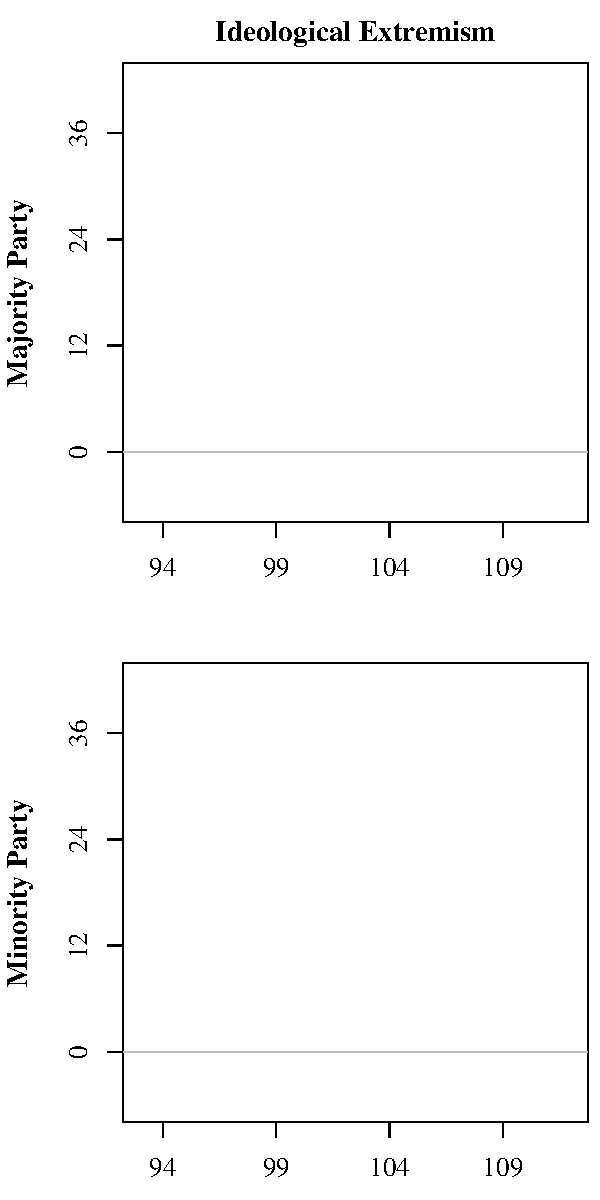
\includegraphics[]{C:/Users/Ethan/Documents/GitHub/partycalls/plots/senate-figure2-emIRT_only.pdf}
	
\end{figure}

\begin{figure}[ht]
	\caption{Ideological Extremism, Senate $ p < 0.05 $}
	\centering
	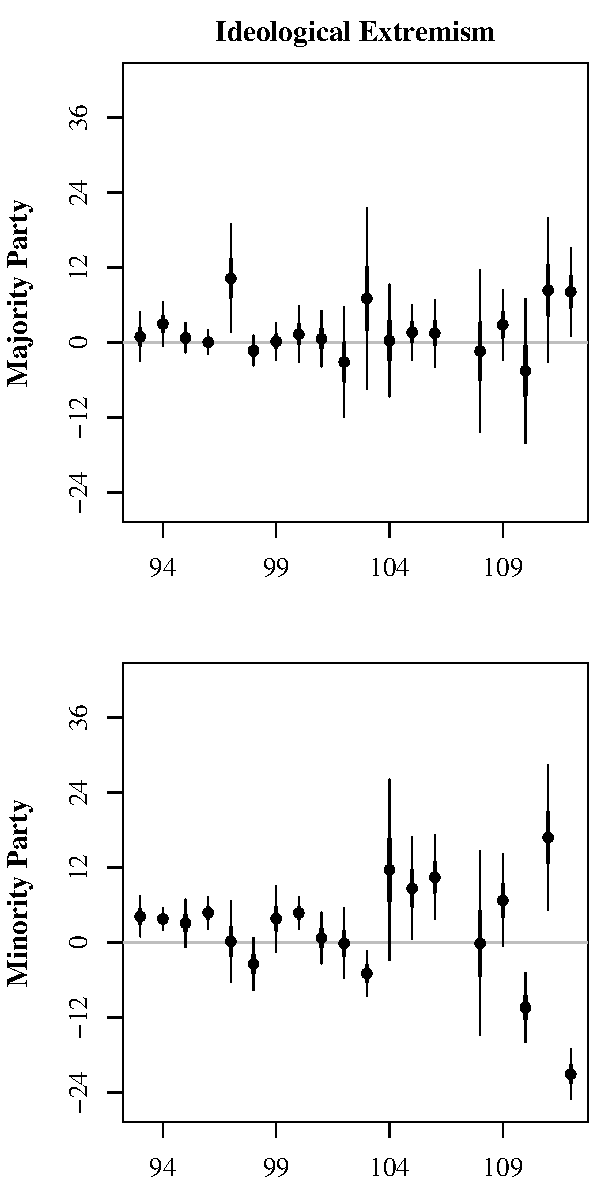
\includegraphics[]{C:/Users/Ethan/Documents/GitHub/partycalls/plots/senate-figure2-p_05.pdf}
	
\end{figure}

\begin{figure}[ht]
	\caption{Figure 2, Ideological Extremism, House}
	\centering
	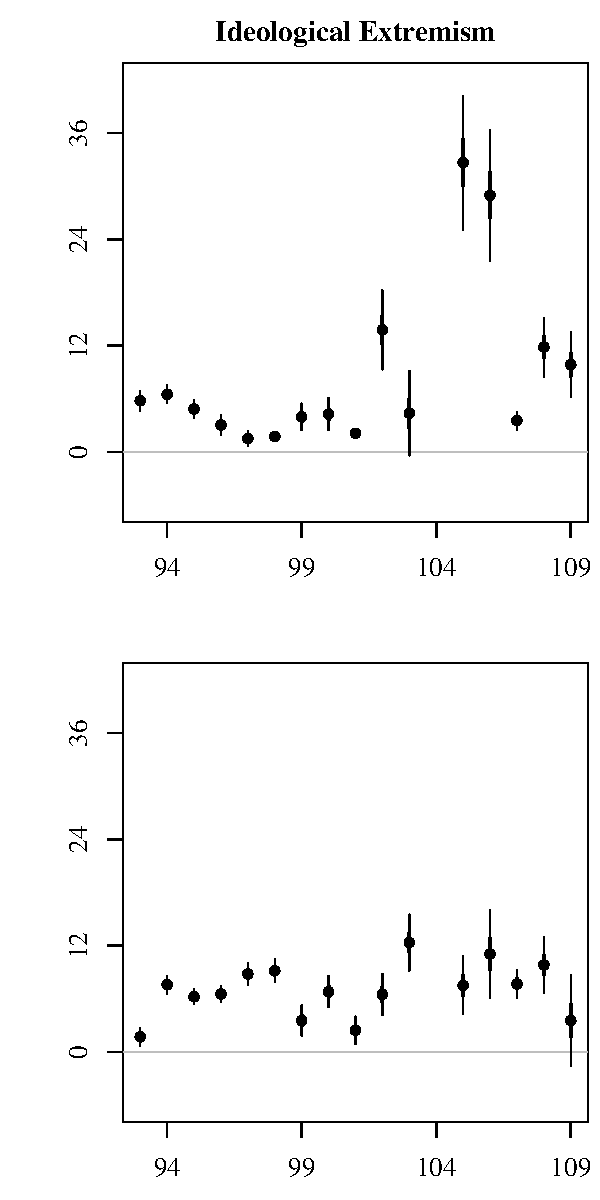
\includegraphics[]{C:/Users/Ethan/Documents/GitHub/partycalls/plots/who-heeds-figure2-replication_emIRT_only.pdf}
	
\end{figure}


\begin{table}
	\begin{center}
		\begin{tabular}{l c c }
			\hline
			& Other Democrats & Southern Democrats \\
			\hline
			ideological\_extremism & $-2.913^{***}$ & $-6.115^{***}$ \\
			& $(0.780)$      & $(1.449)$      \\
			chair                  & $-1.839^{**}$  & $-1.056$       \\
			& $(0.690)$      & $(1.634)$      \\
			pfrate100              & $0.809^{***}$  & $0.848^{***}$  \\
			& $(0.042)$      & $(0.066)$      \\
			pres\_vote\_share      & $32.148^{***}$ & $27.069^{***}$ \\
			& $(3.298)$      & $(6.069)$      \\
			vote\_share            & $-7.566^{*}$   & $-3.953$       \\
			& $(3.404)$      & $(4.469)$      \\
			power\_committee       & $-0.443$       & $0.903$        \\
			& $(0.968)$      & $(2.389)$      \\
			female                 & $-0.315$       & $-2.158$       \\
			& $(0.909)$      & $(2.310)$      \\
			afam                   & $4.058$        &                \\
			& $(3.060)$      &                \\
			latino                 & $-0.759$       &                \\
			& $(2.564)$      &                \\
			up\_for\_reelection    & $-0.656$       & $-1.556$       \\
			& $(0.523)$      & $(1.248)$      \\
			seniority              & $-0.004$       & $-0.005$       \\
			& $(0.077)$      & $(0.186)$      \\
			freshman               & $-1.170$       & $1.653$        \\
			& $(0.725)$      & $(1.687)$      \\
			retiree                & $2.525^{*}$    & $2.213$        \\
			& $(1.164)$      & $(2.613)$      \\
			best\_committee        & $0.114$        & $0.530$        \\
			& $(0.166)$      & $(0.354)$      \\
			leader                 & $-0.545$       & $-2.463$       \\
			& $(0.868)$      & $(2.613)$      \\
			(Intercept)            & $6.579$        & $-5.079$       \\
			& $(3.807)$      & $(7.180)$      \\
			\hline
			R$^2$                  & 0.551          & 0.614          \\
			Adj. R$^2$             & 0.543          & 0.592          \\
			Num. obs.              & 793            & 244            \\
			RMSE                   & 6.664          & 8.531          \\
			\hline
			\multicolumn{3}{l}{\scriptsize{$^{***}p<0.001$, $^{**}p<0.01$, $^*p<0.05$}}
		\end{tabular}
		\caption{Senate $ p < 0.01 $}
		\label{table:coefficients}
	\end{center}
\end{table}


\begin{table}
	\begin{center}
		\begin{tabular}{l c c }
			\hline
			& Other Democrats & Southern Democrats \\
			\hline
			ideological\_extremism & $0.179$        & $-3.569^{**}$ \\
			& $(0.638)$      & $(1.266)$     \\
			chair                  & $0.139$        & $0.110$       \\
			& $(0.582)$      & $(1.464)$     \\
			pfrate100              & $0.749^{***}$  & $0.964^{***}$ \\
			& $(0.035)$      & $(0.060)$     \\
			pres\_vote\_share      & $21.199^{***}$ & $12.636^{*}$  \\
			& $(2.785)$      & $(5.456)$     \\
			vote\_share            & $-5.848^{*}$   & $-2.366$      \\
			& $(2.875)$      & $(4.013)$     \\
			power\_committee       & $-1.666^{*}$   & $-0.023$      \\
			& $(0.816)$      & $(2.146)$     \\
			female                 & $-0.604$       & $-6.544^{**}$ \\
			& $(0.767)$      & $(2.075)$     \\
			afam                   & $3.260$        &               \\
			& $(2.583)$      &               \\
			latino                 & $-2.173$       &               \\
			& $(2.165)$      &               \\
			up\_for\_reelection    & $-0.662$       & $-0.899$      \\
			& $(0.441)$      & $(1.119)$     \\
			seniority              & $-0.140^{*}$   & $-0.062$      \\
			& $(0.065)$      & $(0.167)$     \\
			freshman               & $-1.617^{**}$  & $-0.169$      \\
			& $(0.612)$      & $(1.510)$     \\
			retiree                & $2.417^{*}$    & $0.467$       \\
			& $(0.982)$      & $(2.344)$     \\
			best\_committee        & $0.270$        & $0.224$       \\
			& $(0.140)$      & $(0.317)$     \\
			leader                 & $0.082$        & $-2.144$      \\
			& $(0.733)$      & $(2.346)$     \\
			(Intercept)            & $12.495^{***}$ & $-4.481$      \\
			& $(3.178)$      & $(6.527)$     \\
			\hline
			R$^2$                  & 0.606          & 0.698         \\
			Adj. R$^2$             & 0.598          & 0.681         \\
			Num. obs.              & 793            & 244           \\
			RMSE                   & 5.625          & 7.650         \\
			\hline
			\multicolumn{3}{l}{\scriptsize{$^{***}p<0.001$, $^{**}p<0.01$, $^*p<0.05$}}
		\end{tabular}
		\caption{Senate $ p < 0.05 $}
	\end{center}
\end{table}




\end{document}